\begin{SCn}

\scnsectionheader{\currentname}

\scnstartsubstruct

\scnheader{Предметная область входящих в ostis-систему и выходящих из ostis-системы сообщений}
\scnsdmainclass{сообщение}
\scnsdclass{***}
\scnsdrelation{декомпозиция сообщения; последовательность сообщений*; отправитель*; получатель*}

\scnheader{сообщение}
\scnidtf{дискретная информационная конструкция, используемая в процессе передачи от \textit{\textbf{отправителя*}} к \textit{\textbf{получателю*}}}
\scnsubset{дискретная информационная конструкция}
\scnsubdividing{сообщение пользователя системы\\
\scnaddlevel{1}
\scnidtf{сообщение, \textit{\textbf{отправителем*}} которого является пользователь системы}
\scnsuperset{сообщение пользователя ostis-системы}
\scnaddlevel{-1}; сообщение системы}
\scnsubdividing{атомарное сообщение; 
неатомарное сообщение\\
\scnaddlevel{1}
\scnidtf{сообщение, в состав которого входят другие сообщения}
\scnrelfrom{типичная семантическая окрестность}{
\scnfilelong{
\begin{figure}[H]
\centering
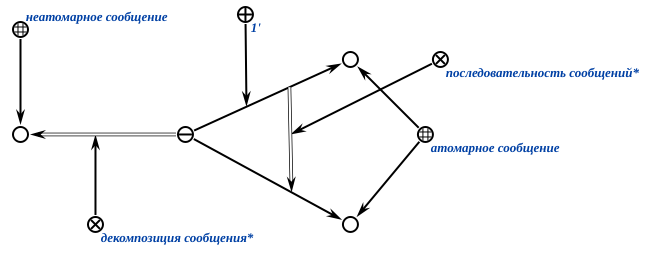
\includegraphics[width=0.7\linewidth]{figures/chapter2/sd_ostis_sys_models/sd_osi/non_atomic_message.png}
\end{figure}
}}
\scnaddlevel{-1}}
\scnsubdividing{сообщение на естественном языке
\scnaddlevel{1}
\scnidtf{сообщение, написанное с использованием естественного языка}
\scnrelfrom{типичная семантическая окрестность}{
\scnfilelong{
\begin{figure}[H]
\centering
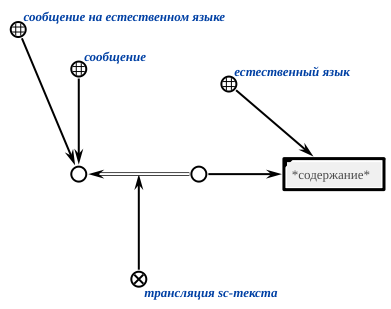
\includegraphics[width=0.4\linewidth]{figures/chapter2/sd_ostis_sys_models/sd_osi/natural_language_message.png}
\end{figure}
}}
\scnaddlevel{-1};
сообщение на искусственном языке\\
\scnaddlevel{1}
\scnidtf{сообщение, написанное с использованием искусственного языка}
\scnrelfrom{типичная семантическая окрестность}{
\scnfilelong{
\begin{figure}[H]
\centering
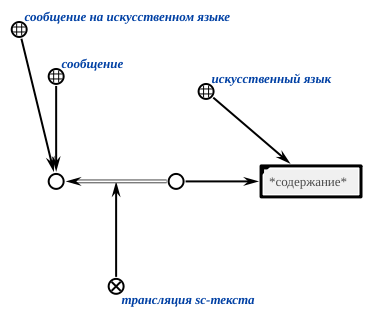
\includegraphics[width=0.4\linewidth]{figures/chapter2/sd_ostis_sys_models/sd_osi/artificial_language_message.png}
\end{figure}
}}
\scnaddlevel{-1}}
%=================
\scnsuperset{графическое сообщение
\scnaddlevel{1}
\scnidtf{сообщение, содержащее графическую информацию}
\scnsuperset{видео-сообщение}
\scnaddlevel{1}
\scnidtf{сообщение, содержащее видео-информацию}
\scnrelfrom{типичная семантическая окрестность}{
\scnfilelong{
\begin{figure}[H]
\centering
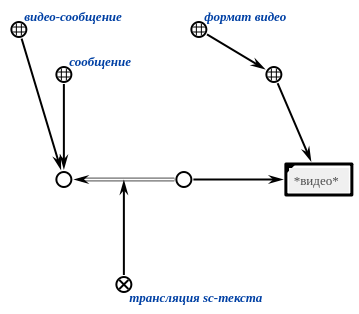
\includegraphics[width=0.4\linewidth]{figures/chapter2/sd_ostis_sys_models/sd_osi/video_message.png}
\end{figure}
}}
\scnaddlevel{-1}
\scnaddlevel{-1}
}
\scnsuperset{аудио-сообщение\\
\scnaddlevel{1}
\scnidtf{сообщение, представленное в звуковом формате}
\scnrelfrom{типичная семантическая окрестность}{
\scnfilelong{
\begin{figure}[H]
\centering
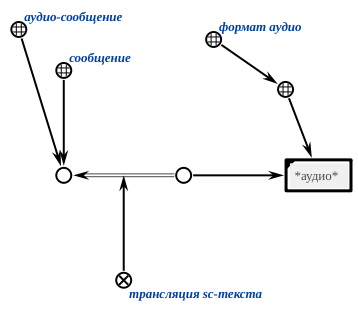
\includegraphics[width=0.4\linewidth]{figures/chapter2/sd_ostis_sys_models/sd_osi/audio_message.png}
\end{figure}
}}
\scnaddlevel{-1}
}
\scnsuperset{обонятельное сообщение\\
\scnaddlevel{1}
\scnidtf{сообщение, содержащее информацию о запахах}
\scnaddlevel{-1}
}
\scnsuperset{текстовое сообщение\\
\scnaddlevel{1}
\scnidtf{сообщение, содержащее текстовую информацию}
\scnrelfrom{типичная семантическая окрестность}{
\scnfilelong{
\begin{figure}[H]
\centering
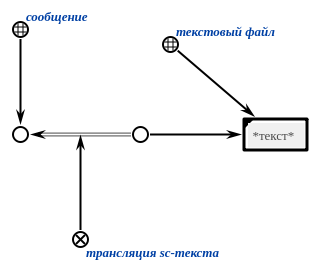
\includegraphics[width=0.4\linewidth]{figures/chapter2/sd_ostis_sys_models/sd_osi/text_message.png}
\end{figure}
}}
\scnaddlevel{-1}
}
\scnsuperset{сообщение, требующее трансляции
\scnaddlevel{1}
\scnidtf{сообщение, которое система должна сформировать для дальнейшей передачи его пользователю}
\scnaddlevel{-1}}
\scnsuperset{протранслированное сообщение
\scnaddlevel{1}
\scnidtf{сообщение, которое было сформировано системой для дальнейшей передачи его пользователю}
\scnaddlevel{-1}}

%Разбиение по признаку автора сообщения
\scnheader{сообщение пользователя ostis-системы}
\scnidtf{сообщение, \textit{\textbf{отправителем*}} которого является пользователь ostis-системы}
\scnsubdividing{сообщение пользователя на внешнем языке\\
\scnaddlevel{1}
\scnidtf{сообщение пользователя ostis-системы, сформированное на языке, внешнем по отношению к ostis-системе, который не используется для коммуникации внутри системы}
\scnsuperset{сообщение пользователя на языке интерфейсных действий}
\scnaddlevel{1}
\scnidtf{сообщение пользователя ostis-системы, сформированное на языке интерфейсных действий (интерфейсных команд), представляющее собой последовательность действий с указанием объектов, на которых эти действия заданы, и типов действий}
\scnaddlevel{-1}
\scnaddlevel{-1}; 
сообщение пользователя на внутреннем языке\\
\scnaddlevel{1}
\scnidtf{сообщение пользователя, записаннное в SC-коде}
\scnidtf{сообщение пользователя ostis-системы, представляющее собой некоторый sc-текст, предназначенный для анализа ostis-системой}
\scnaddlevel{-1}}
\scnrelfrom{типичная семантическая окрестность}{
\scnfilelong{
\begin{figure}[H]
\centering
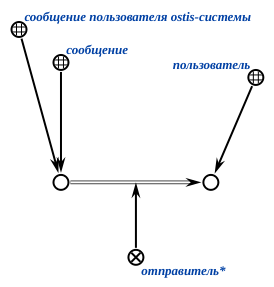
\includegraphics[width=0.35\linewidth]{figures/chapter2/sd_ostis_sys_models/sd_osi/user_message.png}
\end{figure}
}}

\scnheader{сообщение системы}
\scnidtf{сообщение, \textit{\textbf{отправителем*}} которого является некоторая система}
\scnsuperset{сообщение ostis-системы}

\scnheader{сообщение ostis-системы}
\scnidtf{сообщение, \textit{\textbf{отправителем*}} которого является ostis-система}
\scnsubdividing{эффекторное сообщение ostis-системы; рецепторное сообщение ostis-системы}
\scnrelfrom{типичная семантическая окрестность}{
\scnfilelong{
\begin{figure}[H]
\centering
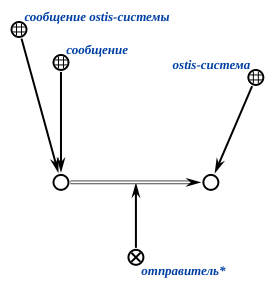
\includegraphics[width=0.35\linewidth]{figures/chapter2/sd_ostis_sys_models/sd_osi/ostis_system_message.png}
\end{figure}
}}

%Разбиение по признаку адресата сообщения
\scnheader{эффекторное сообщение ostis-системы}
\scnidtf{сообщение ostis-системы, формируемое самой ostis-системой при возникновении некоторых ситуаций}
\scnnote{К ситуациям, инициирующим возникновение эффекторных сообщений, можно отнести:
\begin{scnitemize}
    \item {ситуации, возникающие при анализе деятельности самого пользователя. Например, задание аргументов, не соответствующих типу инициируемого действия или появление подсказок при использовании компонентов пользовательского интерфейса;}
    \item {ситуации, возникающие при анализе синтаксиса текстов внешних языков. Например, неполнота сформированного предложения на внешнем языке или использование конструкций, нехарактерных или некорректно использованных в контексте отдельно взятого внешнего языка.}
\end{scnitemize}}

\scnheader{рецепторное сообщение ostis-системы}
\scnidtf{сообщение ostis-системы, являющееся реакцией на императивное сообщение}
\scnnote{Возможными реакциями ostis-системы на императивное сообщение пользователя являются:
\begin{scnitemize}
    \item {указание факта завершения выполнения некоторой задачи, что, например, характерно для поведенческих действий;}
    \item {получение ответа* на поставленную задачу, формируемого либо в результате анализа базы знаний пользовательского интерфейса, либо в результате анализа предметной части базы знаний самой ostis-системы.}
\end{scnitemize}}

%Разбиение по атомарности
\scnheader{атомарное сообщение}
\scnidtf{сообщение, в состав которого не входят другие сообщения}
\scnsubdividing{вопросительное сообщение; императивное сообщение; повествовательное сообщение}
\scnsubdividing{сообщение без эмоциональной окраски\\
\scnaddlevel{1}
\scnidtf{атомарное сообщение, не выражающее какую-либо эмоцию}
\scnaddlevel{-1}; 
сообщение, имеющее эмоциональную окраску}
\scnsubdividing{сообщение о прошлом
\scnaddlevel{1}
\scnidtf{атомарное сообщение, содержащее информацию о прошлом}
\scnaddlevel{-1}; 
сообщение о настоящем
\scnaddlevel{1}
\scnidtf{атомарное сообщение, содержащее информацию о настоящем}
\scnaddlevel{-1}; 
сообщение о будушем
\scnaddlevel{1}
\scnidtf{атомарное сообщение, содержащее информацию о будущем}
\scnaddlevel{-1}}

\scnheader{вопросительное сообщение}
\scnidtf{атомарное сообщение, выражающее вопрос}
\scnsuperset{сообщение запроса информации\\
\scnaddlevel{1}
\scnidtf{атомарное сообщение, являющееся запросом какой-либо новой информации}
\scnaddlevel{-1}}

\scnheader{императивное сообщение}
\scnidtf{атомарное сообщение, побуждающее к какому-либо действию}
\scnsuperset{сообщение пожелания\\
\scnaddlevel{1}
\scnidtf{императивное сообщение, содержащее какое-либо пожелание}
\scnaddlevel{-1}}

\scnheader{повествовательное сообщение}
\scnidtf{атомарное сообщение, предназначенное для передачи информации об \textit{\textbf{объекте\scnrolesign}} сообщения}
\scnsubdividing{информационное сообщение; 
нейтральное сообщение
\scnaddlevel{1}
\scnidtf{повествовательное сообщение, не несущее новой информации и не подверждающее/отрицающее ранее известную информацию}
\scnnote{Примером нейтрального сообщения является сообщение, содержащее ранее известную системе информацию, но не являющееся ответом на вопрос, заданный для подтверждения/отрицания этой информации.}
\scnsuperset{привественное сообщение
\scnaddlevel{1}
\scnidtf{нейтральное сообщение, являющееся приветствием}
\scnaddlevel{-1}}
\scnsuperset{прощальное сообщение
\scnaddlevel{1}
\scnidtf{нейтральное сообщение, являющееся прощанием}
\scnaddlevel{-1}}
\scnaddlevel{-1}}
\scnrelfrom{типичная семантическая окрестность}{
\scnfilelong{
\begin{figure}[H]
\centering
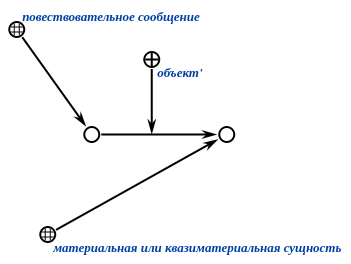
\includegraphics[width=0.4\linewidth]{figures/chapter2/sd_ostis_sys_models/sd_osi/narrative_message.png}
\end{figure}
}}


\scnheader{информационное сообщение}
\scnidtf{повествовательное сообщение, предназначенное для передачи новой информации об \textit{\textbf{объекте\scnrolesign}} сообщения}
\scnsubdividing{сообщение информирования; 
сообщение отрицания информации
\scnaddlevel{1}
\scnidtf{информационное сообщение, отрицающее какую-либо ранее известную информацию}
\scnaddlevel{-1};
сообщение подтверждения информации
\scnaddlevel{1}
\scnidtf{информационное сообщение, подтверждающее какую-либо ранее известную информацию}
\scnaddlevel{-1}}

\scnheader{сообщение информирования}
\scnidtf{информационное сообщение, предназначенное для передачи ранее неизвестной информации об \textit{\textbf{объекте\scnrolesign}} сообщения}
\scnsuperset{сообщение информирования о достижениях\\
\scnaddlevel{1}
\scnidtf{сообщение информирования, предназначенное для оповещения о достижениях \textit{\textbf{объекта\scnrolesign}} сообщения}
\scnaddlevel{-1}}
\scnsuperset{сообщение информирования о местоположении\\
\scnaddlevel{1}
\scnidtf{сообщение информирования, предназначенное для оповещения о местоположении \textit{\textbf{объекта\scnrolesign}} сообщения}
\scnaddlevel{-1}}
\scnsuperset{сообщение информирования об отношении\\
\scnaddlevel{1}
\scnidtf{сообщение информирования, предназначенное для оповещения о связи \textit{\textbf{объекта\scnrolesign}} сообщения с иной сущностью}
\scnaddlevel{-1}}
\scnsuperset{сообщение информирования о проблемах\\
\scnaddlevel{1}
\scnidtf{сообщение информирования, предназначенное для оповещения о проблемах \textit{\textbf{объекта\scnrolesign}} сообщения}
\scnaddlevel{-1}}
\scnsuperset{сообщение информирования о состоянии здоровья
\scnaddlevel{1}
\scnidtf{сообщение информирования, предназначенное для оповещения об состоянии здоровья \textit{\textbf{объекта\scnrolesign}} сообщения}
\scnaddlevel{-1}}

\scnheader{сообщение, имеющее эмоциональную окраску}
\scnidtf{атомарное сообщение, выражающее какую-либо эмоцию}
\scnsubdividing{сообщение, имеющее негативную эмоциональную окраску\\
\scnaddlevel{1}
\scnidtf{атомарное сообщение, выражающее негативную эмоцию}
\scnnote{К негативным эмоциям относятся гнев, страх, ненависть, испуг и др.}
\scnaddlevel{-1};
сообщение, имеющее нейтральную эмоциональную окраску\\
\scnaddlevel{1}
\scnidtf{атомарное сообщение, выражающее нейтральную эмоцию}
\scnnote{К нейтральным эмоциям относятся любопытство, удивление, безразличие и др.}
\scnaddlevel{-1};
сообщение, имеющее положительную эмоциональную окраску\\
\scnaddlevel{1}
\scnidtf{атомарное сообщение, выражающее положительную эмоцию}
\scnnote{К положительным эмоциям относятся удовольствие, ликование, любовь и др.}
\scnaddlevel{-1};
сообщение с неопределенной эмоциональной окраской
\scnaddlevel{1}
\scnidtf{атомарное сообщение, имеющее неопределенную эмоциональную окраску, на основе которой трудно определить эмоцию}
\scnnote{Данный тип сообщений может быть вызван в случае, когда человек испытывает сразу несколько, как правило, противоречащих друг другу эмоций.}
\scnaddlevel{-1}}

%\scnheader{время отправления сообщения}
%\scnsubset{начало}
%\scnidtf{временная точка}

%\scnheader{время получения сообщения}
%\scnsubset{завершение}
%\scnidtf{временная точка, в которой сообщение было получено}

%отношения
\scnheader{декомпозиция сообщения*}
\scnidtf{квазибинарное отношение, связывающее неатомарное сообщение c множеством атомарных сообщений, на которое сообщение разделяется}
\scnrelfrom{первый домен}{связь}
\scnrelfrom{второй домен}{неатомарное сообщение}
\scniselement{квазибинарное отношение}
\scniselement{ориентированное отношение}
\scniselement{антирефлексивное отношение}
\scniselement{антитранзитивное отношение}
\scniselement{асимметричное отношение}

\scnheader{последовательность сообщений*}
\scnidtf{бинарное отношение, связывающее упорядоченные относительно друг друга сообщения}
\scnrelfrom{первый домен}{sc-дуга принадлежности}
\scnrelfrom{второй домен}{sc-дуга принадлежности}
\scniselement{бинарное отношение}
\scniselement{ориентированное отношение}
\scniselement{антирефлексивное отношение}
\scniselement{транзитивное отношение}
\scniselement{асимметричное отношение}

\newpage
\scnheader{Рис. Пример использования отношений \textbf{декомпозиция сообщения*} и \textbf{последовательность сообщений*}}
\scneqtable{
\begin{figure}[H]
\centering
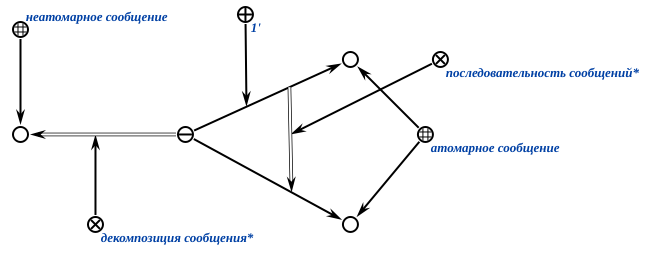
\includegraphics[width=0.7\linewidth]{figures/chapter2/sd_ostis_sys_models/sd_osi/non_atomic_message.png}
\end{figure}
}}

\scnheader{отправитель*}
\scnidtf{отправитель сообщения*}
\scnidtf{бинарное ориентированное отношение, связывающее сообщение с его отправителем*}
\scnrelfrom{первый домен}{сообщение}
\scnrelfrom{второй домен}{живое существо $\cup$ кибернетическая система}
\scniselement{бинарное отношение}
\scniselement{ориентированное отношение}
\scniselement{рефлексивное отношение}
\scniselement{транзитивное отношение}
\scniselement{асимметричное отношение}

\scnheader{получатель*}
\scneq{получатель сообщения*}
\scnidtf{бинарное ориентированное отношение, связывающее сообщение с его получателем*}
\scnrelfrom{первый домен}{сообщение}
\scnrelfrom{второй домен}{живое существо $\cup$ кибернетическая система}
\scniselement{бинарное отношение}
\scniselement{ориентированное отношение}
\scniselement{рефлексивное отношение}
\scniselement{транзитивное отношение}
\scniselement{асимметричное отношение}

\newpage
\scnheader{Рис. Пример использования отношений \textbf{отправитель*} и \textbf{получатель*}}
\scneqtable{
\begin{figure}[H]
\centering
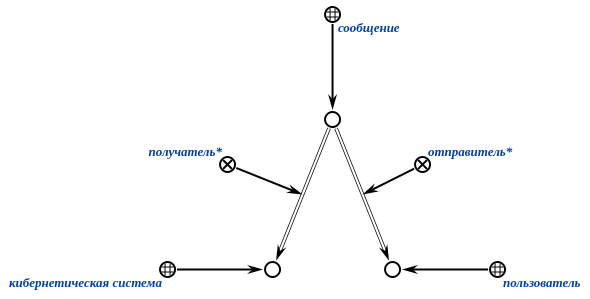
\includegraphics[width=0.7\linewidth]{figures/chapter2/sd_ostis_sys_models/sd_osi/example_of_using_sender_and_recipient.png}
\end{figure}
}}

\end{SCn}
